\section{funzioni iperboliche}

\begin{definition}[funzioni iperboliche]
Le funzioni
\emph{coseno iperbolico} e \emph{seno iperbolico}
sono definite, per ogni $x\in \RR$,
come segue:
\mymargin{$\sinh$, $\cosh$}%
\index{$\sinh$, $\cosh$}%
\index{funzioni!iperboliche}%
\index{seno!iperbolico}%
\index{coseno!iperbolico}%
\index{$\sinh$}%
\index{$\cosh$}%
\begin{equation}
\label{eq:sinh_cosh}
  \cosh x = \frac{e^x + e^{-x}}{2},
  \qquad
  \sinh x = \frac{e^x - e^{-x}}{2}.
\end{equation}
\end{definition}

\begin{theorem}[proprietà delle funzioni iperboliche]
Valgono le seguenti proprietà.
\begin{enumerate}
\item
la funzione $\sinh$ è dispari, $\cosh$ è pari:
\[
\sinh(-x) = -\sinh(x),
\qquad
\cosh(-x) = \cosh(x);
\]

\item
i punti del piano con coordinate $(\cosh x, \sinh x)$
per $x\in \RR$
sono disposti su un ramo di iperbole in quanto vale:
\[
  \cosh^2 x - \sinh^2 x = 1;
\]

\item formule di addizione:
\begin{align*}
  \cosh(\alpha+\beta) &= \cosh \alpha \cosh \beta + \sinh \alpha \sinh \beta,\\
  \sinh(\alpha+\beta) &= \sinh \alpha \cosh \beta + \cosh \alpha \sinh \beta;
\end{align*}

% \item si ha
% \begin{align*}
%   \cosh x
%   &= \sum_{k=0}^{+\infty} \frac{x^{2k}}{(2k)!}
%   = 1 + \frac{x^2}{2} + \frac{x^4}{4!} + \frac{x^6}{6!} + \dots \\
%   \sinh x
%   &= \sum_{k=0}^{+\infty} \frac{x^{2k+1}}{(2k+1)!}
%   = x + \frac{x^3}{6} + \frac{x^5}{5!} + \frac{x^7}{7!} + \dots
% \end{align*}

\item
la funzione $\sinh$ è strettamente crescente su tutto $\RR$,
la funzione $\cosh$
è strettamente crescente sull'intervallo
$[0,+\infty)$ e strettamente decrescente
nell'intervallo $(-\infty,0]$;

\item per $x\to +\infty$ si ha $\sinh x \to +\infty$, $\cosh x \to +\infty$, 
per $x\to -\infty$ si ha $\sinh x \to -\infty$, $\cosh x \to +\infty$.

\end{enumerate}
\end{theorem}

\newsavebox{\qrfigiperb}\sbox{\qrfigiperb}{\myurlhere{figiperb}{funzioni iperboliche}}%
\begin{figure}
  \centering%
  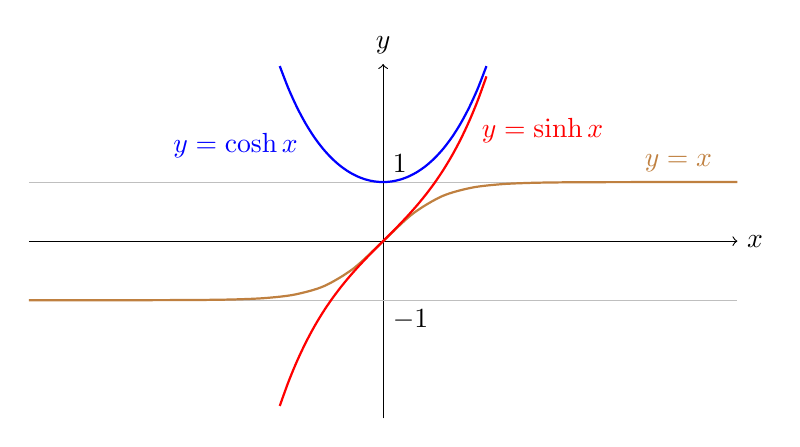
\begin{tikzpicture}[scale=0.75]
  \draw[->] (-6,0) -- (6,0) node[right] {$x$};
  \draw[->] (0,-3) -- (0,3) node[above] {$y$};
  \foreach \y in {1, -1} {
    \draw[shift={(0,\y)},lightgray] (-6,0) -- (6,0);
  }
  \draw (0,1) node [above right] {$1$};
  \draw (0,-1) node [below right] {$-1$};
  \draw[domain=-6:6,smooth,variable=\x,brown,thick] plot ({\x},{tanh(\x)});
  \draw[domain=-1.75:1.75,smooth,variable=\x,blue,thick] plot ({\x},{cosh(\x)});
  \draw[domain=-1.75:1.75,smooth,variable=\x,red,thick] plot ({\x},{sinh(\x)});
  \draw (-2.5,2) node[blue,below] {$y=\cosh x$};
  \draw (2.7,1.5)  node[red,above] {$y=\sinh x$};
  \draw (5,1) node[brown,above] {$y=\tgh x$};
  \end{tikzpicture}
  \caption{%
    I grafici delle funzioni $\sinh$, $\cosh$ e $\tgh$.
    \ifwidemargin\\\\\fi%
    \usebox{\qrfigiperb}%
  }
\end{figure}

\begin{proof}
I primi tre punti si dimostrano facilmente per verifica diretta,
utilizzando la definizione~\eqref{eq:sinh_cosh}.

% Gli sviluppi in serie si ottengono anch'essi sostituendo
% gli sviluppi dell'esponenziale nella definizione.
% Nel $\cosh$ i termini di grado dispari si cancellano, nel $\sinh$ si cancellano
% i termini di grado pari.

Per quanto riguarda la monotonia si osserva che se $x\ge 0$ ogni
addendo delle due serie esposte nel punto 4 è strettamente crescente
(in quanto i coefficienti sono tutti positivi) e dunque le somme delle serie,
cioè la funzione $\cosh$ e la funzione $\sinh$ sono strettamente crescenti
sull'intervallo $[0,+\infty)$. La funzione $\sinh$, essendo dispari,
risulta inoltre crescente anche sull'intervallo $(-\infty,0]$ e quindi
è crescente su tutto $\RR$.

Per l'ultima proprietà basterà usare la definizione~\eqref{eq:sinh_cosh}
e ricordare che (teorema~\ref{th:ordine_infinito})
se $x\to +\infty$ allora
$e^x\to +\infty$ ed $e^{-x}=\frac{1}{e^{x}} \to 0$.
\end{proof}

Osserviamo che $\cosh 0 = 1$ e, per le proprietà di monotonia viste nel teorema
precedente si ha $\cosh x \ge \cosh 0 = 1 > 0$. Dunque $\cosh x$ non si annulla
mai e si può definire per ogni $x\in \RR$ la \emph{tangente iperbolica}
\index{tangente!iperbolica}%
\mymargin{$\tgh$}%
\index{$\tgh$}%
\[
    \tgh x = \frac{\sinh x}{\cosh x}.
\]

La funzione $\sinh\colon \RR\to\RR$ è iniettiva in quanto strettamente crescente ed
è surgettiva in quanto è continua e quindi assume tutti i valori compresi tra
$\lim_{x\to+\infty} \sinh(x) = +\infty$ e $\lim_{x\to -\infty} \sinh(x) = -\infty$. 
Dunque $\sinh\colon \RR \to \RR$
è invertibile e la funzione inversa si chiama \emph{settore di seno iperbolico}
e si denota con
\mymargin{$\settsinh$}%
\index{$\settsinh$}
\index{settore!di seno iperbolico}
\[
    \settsinh \colon \RR \to \RR.
\]
Analogamente la funzione ristretta $\cosh\colon [0,+\infty)\to [1,+\infty)$ è
iniettiva in quanto strettamente crescente ed è surgettiva in quanto
è continua e assume su $[0,+\infty)$ tutti i valori compresi tra $\cosh(0)=1$ e
$\lim_{x\to +\infty} \cosh x = +\infty$.
Dunque la funzione $\cosh x$ ristretta a $[0,+\infty)\to [1,+\infty)$
è invertibile e la funzione inversa si chiama \emph{settore di coseno iperbolico}
\mymargin{$\settcosh$}%
\index{$\settcosh$}
\index{settore!di coseno iperbolico}
\[
    \settcosh \colon [1,+\infty)\to [0,+\infty).
\]

La funzione $\tgh x$ è strettamente crescente su tutto $\RR$ e assume tutti i valori strettamente compresi tra $-1$ e $1$.
La funzione inversa si chiama $\setttgh$.

\begin{exercise}
Fissato $y\in \RR$ si risolva l'equazione
\[
    \frac{e^x - e^{-x}}{2} = y
\]
riconducendola ad una equazione di secondo grado nella variabile $t=e^x$.
Si dimostri quindi che vale
\[
    \settsinh x = \ln\enclose{x + \sqrt{x^2 + 1}}.
\]
In modo analogo si dimostri che vale
\[
    \settcosh x = \ln\enclose{x + \sqrt{x^2 - 1}}
\]
e
\[
    \setttgh x = \ln \sqrt{\frac{1+x}{1-x}}.
\]
\end{exercise}

